\documentclass[]{article}

%%%%%%%%%%%%%%%%%%%
% Packages/Macros %
%%%%%%%%%%%%%%%%%%%
\usepackage{amssymb,latexsym,amsmath}     % Standard packages
\usepackage{graphicx}

%%%%%%%%%%%
% Margins %
%%%%%%%%%%%
\addtolength{\textwidth}{1.0in}
\addtolength{\textheight}{1.00in}
\addtolength{\evensidemargin}{-0.75in}
\addtolength{\oddsidemargin}{-0.75in}
\addtolength{\topmargin}{-.50in}


%%%%%%%%%%%%%%%%%%%%%%%%%%%%%%
% Theorem/Proof Environments %
%%%%%%%%%%%%%%%%%%%%%%%%%%%%%%
\newtheorem{theorem}{Theorem}
\newenvironment{proof}{\noindent{\bf Proof:}}{$\hfill \Box$ \vspace{10pt}}  


%%%%%%%%%%%%
% Document %
%%%%%%%%%%%%
\begin{document}

\title{CS 224n Assignment 2.}
\author{Abhishek Goswami.}
\maketitle

\begin{enumerate}
	\item Written : Understanding word2vec
	
	\begin{enumerate}
		
		\item
		% (a) question on cross entropy
		\begin{equation}
		\sum_{w \in Vocab} y_w \log(\hat{y}_w) = - \log(\hat{y}_o).
		\end{equation}

		because
		
		\begin{equation}
		y_{i} = 
\begin{cases}
    1, & \text{if } i = o\\
    0, & \text{otherwise}
\end{cases}.
		\end{equation}
			
		\item
		% (b) question to compute wrt v_{c}
		\begin{equation}
		\frac{\partial 		\boldsymbol{J}_\textsubscript{naive-softmax}(\boldsymbol{\upsilon}_c, o, \boldsymbol{U})}{\partial \boldsymbol{\upsilon}_c} = 
		- \boldsymbol{u}_{o} + \sum_{w=1}^V \hat{y}_w \boldsymbol{u}_{w}.
		\end{equation}

		also equivalent to 
		
		\begin{equation}
		\frac{\partial 		\boldsymbol{J}_\textsubscript{naive-softmax}(\boldsymbol{\upsilon}_c, o, \boldsymbol{U})}{\partial \boldsymbol{\upsilon}_c} = 
		\boldsymbol{U} (\boldsymbol{\hat{y}} - \boldsymbol{y}).
		\end{equation}
		
		\item
		%  (c) question to compute wrt U
		\begin{equation}
		\frac{\partial 		\boldsymbol{J}_\textsubscript{naive-softmax}(\boldsymbol{\upsilon}_c, o, \boldsymbol{U})}{\partial \boldsymbol{U}} = 
		\boldsymbol{v}_{c} (\boldsymbol{\hat{y}} - \boldsymbol{y})^\top.
		\end{equation}
			
		\item
		%  (d) derivative of sigmoid. 
		\begin{equation}
		\sigma^{\prime}(\boldsymbol{x}) = \sigma(\boldsymbol{x}) (1 - \sigma(\boldsymbol{x}))
		\end{equation}
		
		\item
		%  (e) derivative of neg sample.
		\begin{equation}
		\frac{\partial 		\boldsymbol{J}_\textsubscript{neg-sample}(\boldsymbol{\upsilon}_c, o, \boldsymbol{U})}{\partial \boldsymbol{\upsilon}_c} = 
		(\sigma(\boldsymbol{u}_{o}^\top \boldsymbol{v}_c) - 1) \boldsymbol{u}_{o} -
		\sum_{k=1}^{k} (\sigma(- \boldsymbol{u}_{k}^\top \boldsymbol{v}_c) - 1) \boldsymbol{u}_{k}
		\end{equation}

		\begin{equation}
		\frac{\partial 		\boldsymbol{J}_\textsubscript{neg-sample}(\boldsymbol{\upsilon}_c, o, \boldsymbol{U})}{\partial \boldsymbol{u}_o} = 
		(\sigma(\boldsymbol{u}_{o}^\top \boldsymbol{v}_c) - 1) \boldsymbol{v}_{c}.
		\end{equation}
		
		\begin{equation}
		\frac{\partial 		\boldsymbol{J}_\textsubscript{neg-sample}(\boldsymbol{\upsilon}_c, o, \boldsymbol{U})}{\partial \boldsymbol{u}_k} = 
		-(\sigma(-\boldsymbol{u}_{k}^\top \boldsymbol{v}_c) - 1) \boldsymbol{v}_{c}.
		\end{equation}
		
		$J_\textsubscript{neg-sample}$ is more efficient to compute than $J_\textsubscript{naive-softmax}$. In $J_\textsubscript{naive-softmax}$ we use softmax to compute the probability of outside word given the center word. In order to compute the probability, we need to normalize over all the words in the vocabulary. This is not efficient especially when the vocabulary size is large.
		
		\item
		%  (f) skip gram.
		
		\begin{enumerate}
			\item 
			
		\begin{equation}
		\frac{\partial 		\boldsymbol{J}_\textsubscript{skip-gram}(\boldsymbol{\upsilon}_c, w_{t-m},... w_{t+m}, \boldsymbol{U})}{\partial \boldsymbol{U}} = 
		\sum_{-m \leq j \leq m, j \neq 0} \frac{\partial 		\boldsymbol{J}(\boldsymbol{\upsilon}_c, w_{t+j}, \boldsymbol{U})}{\partial \boldsymbol{U}}.
		\end{equation}
		
      \item
	
		\begin{equation}	
		\frac{\partial 		\boldsymbol{J}_\textsubscript{skip-gram}(\boldsymbol{\upsilon}_c, w_{t-m},... w_{t+m}, \boldsymbol{U})}{\partial \boldsymbol{\upsilon}_{c}} = 
				\sum_{-m \leq j \leq m, j \neq 0} \frac{\partial 		\boldsymbol{J}(\boldsymbol{\upsilon}_c, w_{t+j}, \boldsymbol{U})}{\partial \boldsymbol{v}_{c}}
		\end{equation}	
			
			\item 
		
		\begin{equation}	
		\frac{\partial 		\boldsymbol{J}_\textsubscript{skip-gram}(\boldsymbol{\upsilon}_c, w_{t-m},... w_{t+m}, \boldsymbol{U})}{\partial \boldsymbol{\upsilon}_{w}} = 0, 
		\text{when} w \neq c
		\end{equation}
			
    \end{enumerate}
  
	\end{enumerate}

	\item Coding
	
	\begin{figure}
    \centering
    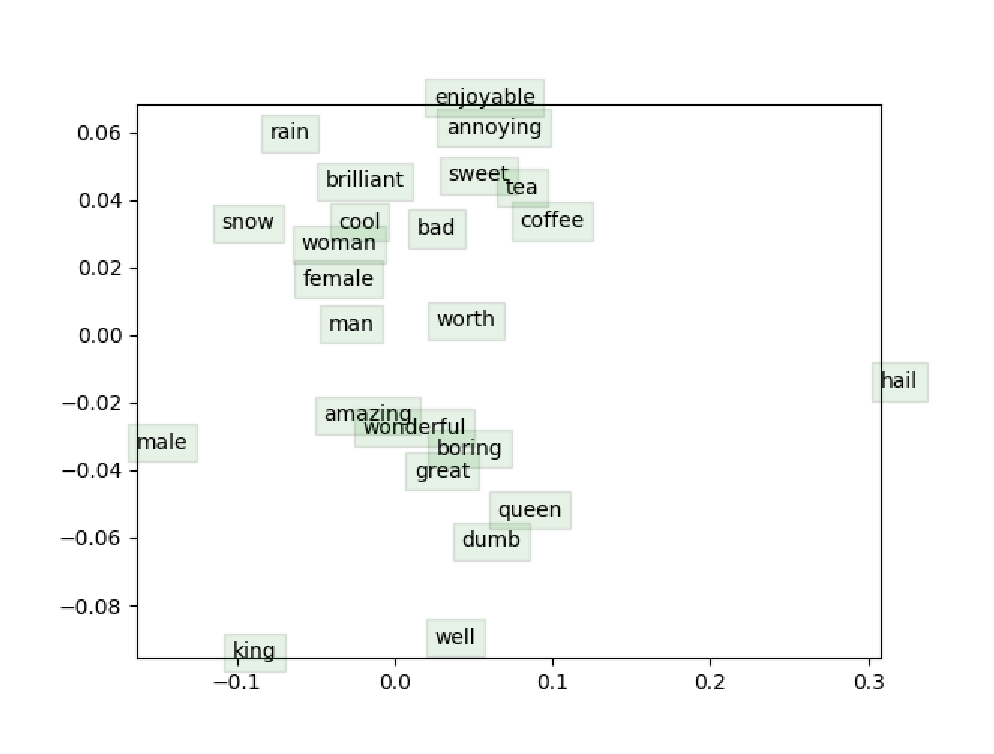
\includegraphics{word_vectors}
    \caption{Word Vectors}
    \label{fig:word_vectors}
	\end{figure}
	
	In Figure ~\ref{fig:word_vectors} we make the following observations :
	\begin{enumerate}
	\item Semantic similarity e.g. (king, male)  (queen, female)
	\item Syntactic structure e.g. (man, woman)  (male, female)
	\item Beverages e.g. (tea, coffee) appear together
	\end{enumerate}
	
\end{enumerate}

\end{document}